\documentclass{article}
\usepackage{pgfplots}
\usepackage{tikz}
\usepgfplotslibrary{fillbetween,groupplots}
\pgfplotsset{compat=1.18}

\begin{document}

\section*{AWS Braket HHL Circuit Depth Experiment Results}

\noindent
\textbf{Device:} SV1 \\
\textbf{Region:} eu-west-2 \\
\textbf{Matrix Sizes:} $N \in \{2, 4, 8, 16\}$ \\
\textbf{Trials per Size:} 20

\vspace{1em}

\begin{figure}[h]
\centering
\resizebox{1\columnwidth}{!}{%
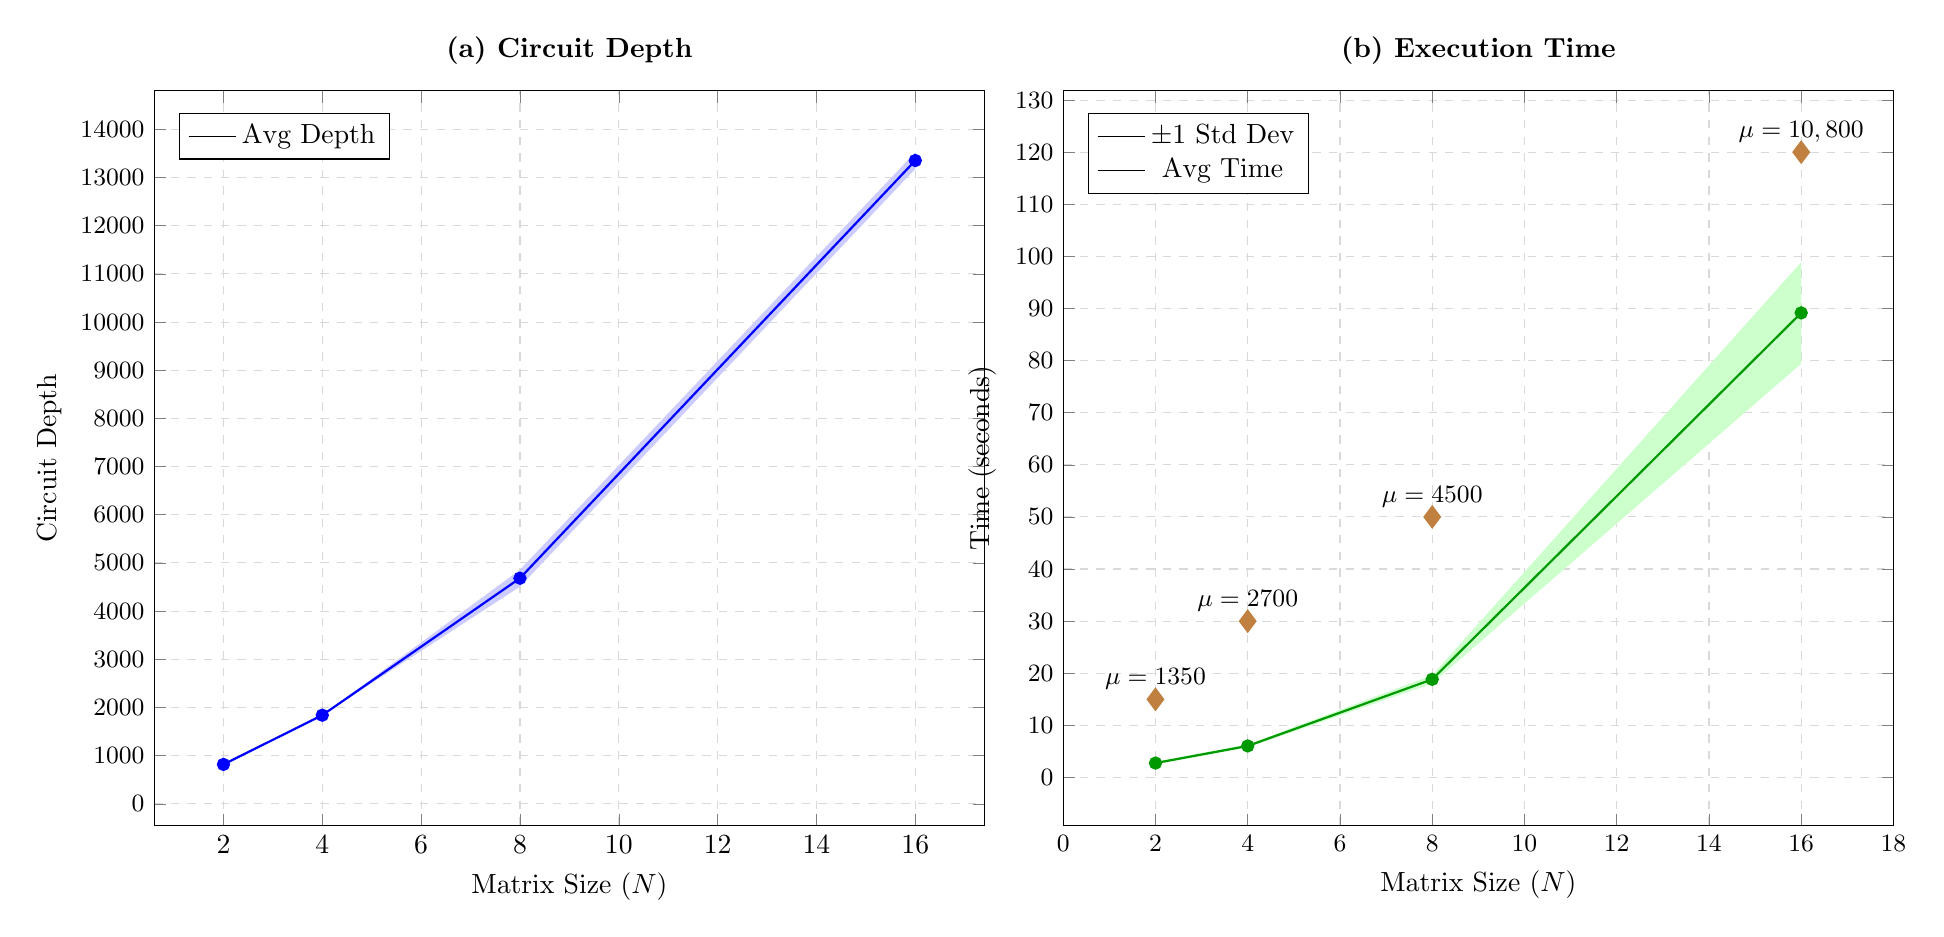
\begin{tikzpicture}
\begin{groupplot}[
    group style={
        group size=2 by 1,
        horizontal sep=1cm,
        vertical sep=2cm,
    },
    width=1\columnwidth,
    height=0.9\columnwidth,
    grid=major,
    grid style={dashed, gray!30},
]

% ===== Plot 1: Circuit Depth (Top-Left) =====
\nextgroupplot[
    xlabel={Matrix Size ($N$)},
    ylabel={Circuit Depth},
    title={\textbf{(a) Circuit Depth}},
    legend pos=north west,
    ytick={0,1000,2000,3000,4000,5000,6000,7000,8000,9000,10000,11000,12000,13000,14000},
    yticklabel style={font=\small, /pgf/number format/.cd, fixed, 1000 sep={}},
    scaled y ticks=false,
]
\addplot[name path=upper,draw=none] coordinates { (2, 817.9) (4, 1839.4) (8, 4858.5) (16, 13527.0) };
\addplot[name path=lower,draw=none] coordinates { (2, 816.4) (4, 1838.8) (8, 4507.2) (16, 13180.3) };
\addplot[blue!20] fill between[of=upper and lower];
\addplot[blue,thick,mark=*] coordinates { (2, 817.1) (4, 1839.1) (8, 4682.9) (16, 13353.6) };
\addlegendentry{Avg Depth}

% ===== Plot 2: Execution Time (Top-Right) =====
\nextgroupplot[
    xlabel={Matrix Size ($N$)},
    ylabel={Time (seconds)},
    title={\textbf{(b) Execution Time}},
    legend pos=north west,
    ytick={0,10,20,30,40,50,60,70,80,90,100,110,120,130,140},
    yticklabel style={font=\small, /pgf/number format/.cd, fixed, 1000 sep={}},
    xticklabel style={font=\small},
    xmin=0, xmax=18,
]
\addplot[name path=upper,draw=none] coordinates { (2, 3.0375) (4, 6.3391) (8, 19.6287) (16, 98.9039) };
\addplot[name path=lower,draw=none] coordinates { (2, 2.4996) (4, 5.7629) (8, 18.0359) (16, 79.4126) };
\addplot[green!20,area legend] fill between[of=upper and lower];
\addlegendentry{$\pm 1$ Std Dev}
\addplot[green!60!black,thick,mark=*] coordinates { (2, 2.7685) (4, 6.0510) (8, 18.8323) (16, 89.1582) };
\addlegendentry{Avg Time}
\addplot[brown,only marks,mark=diamond*,mark size=4pt,forget plot] coordinates { (2, 15.00) (4, 30.00) (8, 50.00) (16, 120.00) };
% Add T value labels
\node[font=\small] at (axis cs:2,15.00) [above] {$\mu=1350$};
\node[font=\small] at (axis cs:4,30.00) [above] {$\mu=2700$};
\node[font=\small] at (axis cs:8,50.00) [above] {$\mu=4500$};
\node[font=\small] at (axis cs:16,120.00) [above] {$\mu=10,800$};
\end{groupplot}
\end{tikzpicture}
}
\caption{AWS Braket Enhanced Hybrid HHL experiment (a) Circuit depth scaling with matrix size, showing a strong relationship between the two factors. (b) The average running time of the HHL circuit for different $N$ and the corresponding $\mu$ for the timelock puzzle that ensures it is solved only after the HHL circuit is complete.}
\end{figure}

\vspace{1em}

\begin{figure}[h]
\centering
\resizebox{1\columnwidth}{!}{%
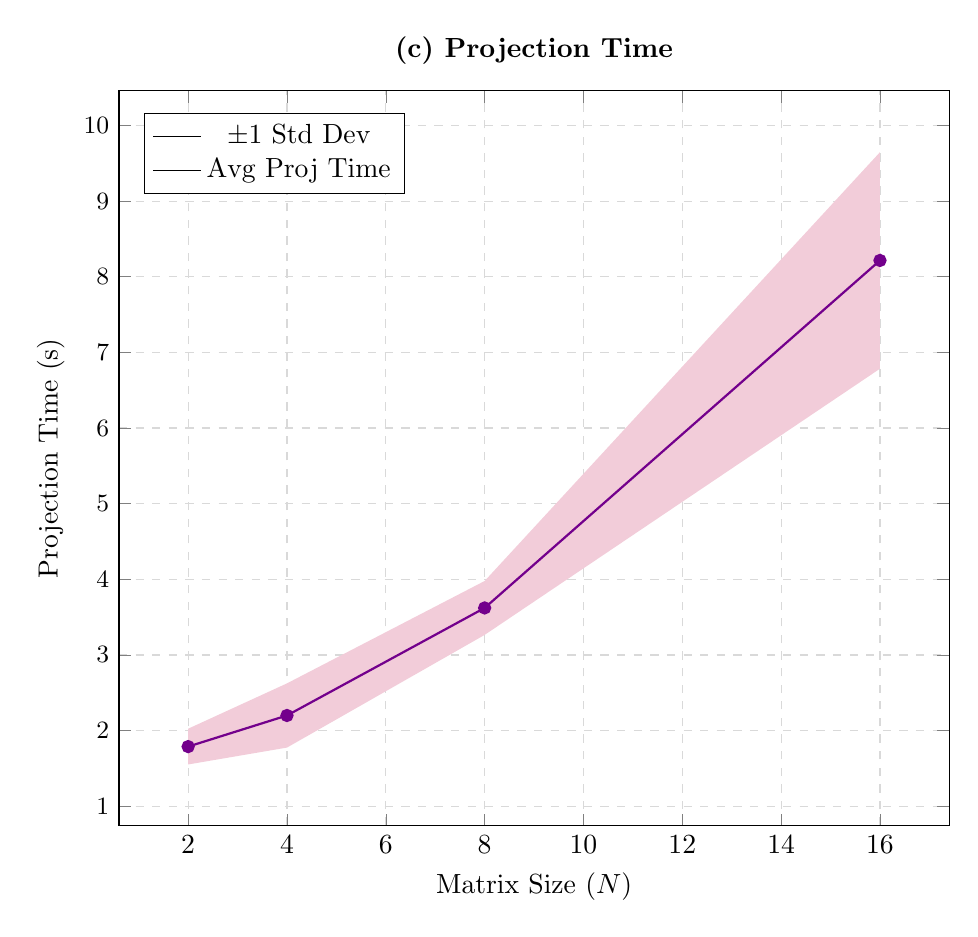
\begin{tikzpicture}
\begin{axis}[
    width=1\columnwidth,
    height=0.9\columnwidth,
    grid=major,
    grid style={dashed, gray!30},
    xlabel={Matrix Size ($N$)},
    ylabel={Projection Time (s)},
    title={\textbf{(c) Projection Time}},
    legend pos=north west,
    ytick={0,1,2,3,4,5,6,7,8,9,10},
    yticklabel style={font=\small},
]
\addplot[name path=upper,draw=none] coordinates { (2, 2.0251) (4, 2.6245) (8, 3.9781) (16, 9.6466) };
\addplot[name path=lower,draw=none] coordinates { (2, 1.5524) (4, 1.7755) (8, 3.2653) (16, 6.7842) };
\addplot[purple!20,area legend] fill between[of=upper and lower];
\addlegendentry{$\pm 1$ Std Dev}
\addplot[purple!60!blue,thick,mark=*] coordinates { (2, 1.7887) (4, 2.2000) (8, 3.6217) (16, 8.2154) };
\addlegendentry{Avg Proj Time}
\end{axis}
\end{tikzpicture}
}
\caption{Individual projection measurement times across different matrix sizes.}
\end{figure}

\vspace{1em}

\subsection*{Key Findings Summary}

\begin{itemize}
    \item \textbf{Circuit depth:} 817 to 13354 (16.3$\times$ increase)
    \item \textbf{Fidelity:} 0.807 to 0.999 (avg: 0.926)
    \item \textbf{Execution time:} 2.77s to 89.16s (32.2$\times$ increase)
\end{itemize}

\end{document}
